% begin module function-def
\begin{frame} \


\psset{xunit=1.1cm,yunit=1.1cm}
\begin{pspicture}(-1,-1)(4,3)
\tiny
\psaxes[labels=none, ticks=none]{->}(0,0)(-0.5,-0.5)(4,3)
\rput[r](0,3){$y$}
\rput[l](4,0){$x$}
\psplot[linecolor=red]{0.5}{3}{0.2 x 2 exp mul 0.5 180 x mul sin mul 0.333333 add add
 }
\rput( 3, 2.5){$y=f(x)$}

\only<2>{
\psline[linecolor=red, linewidth=2pt]{<->}(0.5, 0)(3,0)
\rput(1.75, -0.3){\color{red}Domain}
}

\only<3>{
\psline[linecolor=blue, linewidth=2pt]{<->}(0, -0.5)(0,3)
\rput[l](0.05, 2.35){\color{blue}Co-Domain}
}

\only<4>{
\psline[linecolor=purple, linewidth=3pt]{<->}(0, 0.245)(0,2.205)
\rput[l](0.05, 1.1){\color{purple}Range}
\psline[linestyle=dashed](0,0.245)(1.4, 0.245)
\psline[linestyle=dashed](0,2.205)(2.75, 2.205)
}
\only<5>{
\psline[linewidth=1pt]{<->}(2.166666667, 0)(2.166666667, 1.522222)
\rput[l](2.2,0.7){$f(x)$}
}
\end{pspicture}
%\ \only<handout:0| 1>{%
%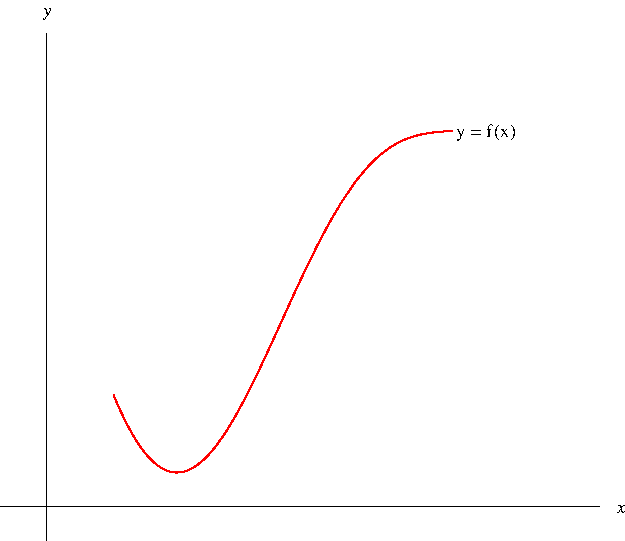
\includegraphics[height=5cm]{precalculus/pictures/01-01-function.pdf}
%}%
%\only<handout:1| 2>{%
%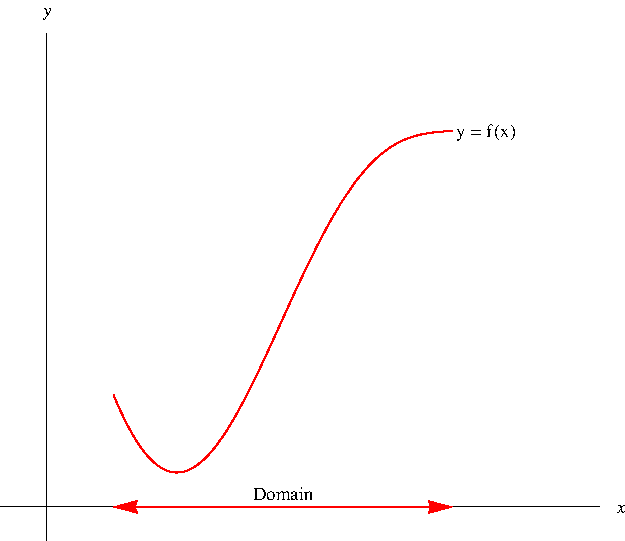
\includegraphics[height=5cm]{precalculus/pictures/01-01-domain.pdf}
%}%
%\only<handout:2| 3>{%
%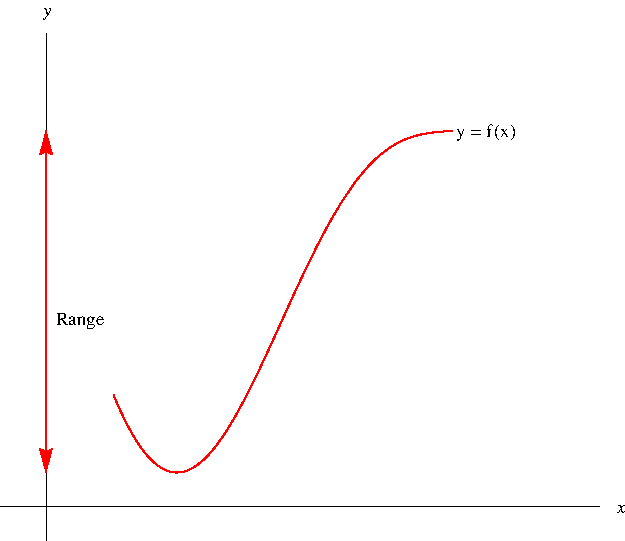
\includegraphics[height=5cm]{precalculus/pictures/01-01-range.pdf}
%}%
%\only<handout:3-| 4->{%
%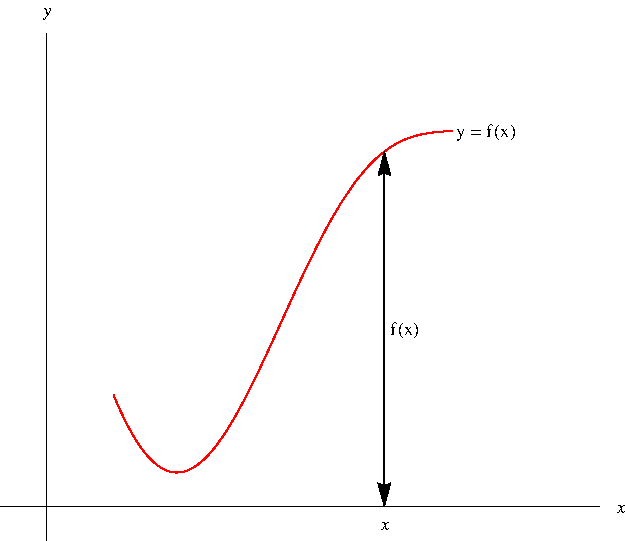
\includegraphics[height=5cm]{precalculus/pictures/01-01-fofx.pdf}
%}%

\begin{definition}[Function]
A function $f$ is a rule that assigns to each element $x$ in a set $D$ exactly one element, called $f(x)$, in a set $E$.
\end{definition}

\only<handout:3| 4>{
\begin{definition}[Range]
The set of all possible values taken by $f(x)$ as the element $x$ runs over elements of $D$ is called the range of $f$. 
\end{definition}
}

\only<handout:1| 2>{
\begin{definition}[Domain]
The set $D$ is called the domain. 
\end{definition}
}

\only<handout:2| 3>{
\begin{definition}[Co-domain]
The set $E$ is called the co-domain. 
\end{definition}
}

\only<handout:4| 5->{
\begin{definition}[Value of $f$ at $x$]
The number $f(x)$ is called the value of $f$ at $x$, and is read ``$f$ of $x$.''
\end{definition}
}

\uncover<4>{}
~\\~\\~\\~\\~\\~



\end{frame}
% end module function-def